%% ---------------------------------------------------------------------------------------------------------------------

\chapter{\textit{go-safer}: Detecting Unsafe Misuses}\label{ch:go-safer}

Another major contribution of this thesis is the development of \toolSafer{}, a \toolVet{}-style, open-source linter
tool with a focus on the \unsafe{} \acrshort{API} in Go.
It can identify some of the insecure code patterns described in Chapter~\ref{ch:unsafe-security-problems} and thus help
developers to write safer code.
This chapter describes the design and implementation of \toolSafer{}, and presents an evaluation of its effectiveness
both using the labeled data set of \unsafe{} usages presented in the previous chapter and a manual analysis of
open-source Go packages.
Figure~\ref{fig:outline5} shows the organization of the contents of this chapter.

\begin{figure}[htp!]
    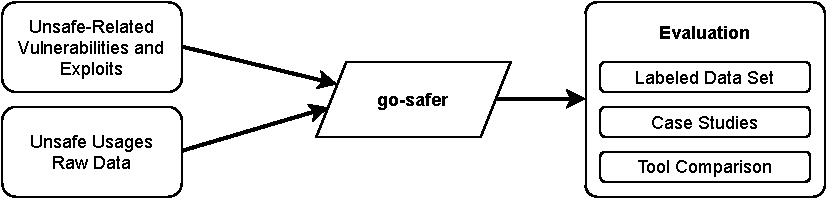
\includegraphics[width=\textwidth]{assets/figures/chapter5/outline5.pdf}
    \caption{Role of Chapter 5 in the thesis outline}
    \label{fig:outline5}
\end{figure}



%% ---------------------------------------------------------------------------------------------------------------------

\section{Design}\label{sec:go-safer:design}

The \toolSafer{} static analysis tool is designed as a linter to identify \checkNum{two} misuses of the \unsafe{}
\acrshort{API} that were previously undetected with existing tools such as \toolVet{} and \toolGosec{}.
The selection of the code patterns that are detected is based on the \unsafe{} usage examples identified using
\toolGeiger{} in popular open-source Go projects as described in
Section~\ref{ch:go-geiger:qualitative-evaluation:labeled-dataset}, as well as the manual analysis of possible
vulnerabilities related to the use of the \unsafe{} \acrshort{API} presented in
Chapter~\ref{ch:unsafe-security-problems}.
The first is the incorrect conversion pattern between slices and strings by creating their header structures as
composite literals as described in Section~\ref{subsec:unsafe-security-problems:slice-casts:gc-race}.
Listing~\ref{lst:go-safer-sliceheader-pass} shows a code example that uses this unsafe pattern.
The insecure creation of a \textit{reflect.SliceHeader} instance is done in Lines~3--7.

\begin{lstlisting}[language=Golang, float, label=lst:go-safer-sliceheader-pass, caption=First vulnerable code pattern detected by \toolSafer{}]
func unsafeFunction(s string) []byte {
    sH := (*reflect.StringHeader)(unsafe.Pointer(&s))
    bH := &reflect.SliceHeader{
        Data: sH.Data,
        Len:  sH.Len,
        Cap:  sH.Len,
    }
    return *(*[]byte)(unsafe.Pointer(bH))
}
\end{lstlisting}


In addition to composite literals of type \textit{reflect.SliceHeader} and \textit{reflect.StringHeader}, \toolSafer{}
analyzes accesses to fields of existing instances of these types.
When they are detected, the tool checks whether the given header structure instance was derived by cast from a real
slice or string.
If that is not the case or can not be statically inferred, for example, because the header value is given as a function
parameter or return type, or there is only a declaration of the variable and type without an initialization, the
field access is treated as potentially unsafe and \toolSafer{} generates a warning.
\toolSafer{} parses the packages to acquire the abstract syntax trees (\acrshort{AST}) for all files.
This allows the tool to run analysis steps that are independent of concrete names in the source code.
If the slice or string header types are renamed to a different type name in the source code, field accesses and
composite literals of the new type name are recognized just like the original types.

The second misuse that \toolSafer{} detects is a direct conversion between struct types containing incompatible types
with architecture-dependent sizes as described in
Section~\ref{subsec:unsafe-security-problems:slice-casts:escape-analysis}.
Listing~\ref{lst:go-safer-structcast-pass} shows an example of such code.
Here, Line~8 contains an incorrect cast between the incompatible structures \textit{A} (Lines~1--3) and \textit{B}
(Lines~4--6).

\begin{lstlisting}[language=Golang, label=lst:go-safer-structcast-pass, caption=Second vulnerable code pattern detected by \toolSafer{}]
type A struct {
    x int
}
type B struct {
    y int64
}
func unsafeFunction(a A) B {
    return *(*B)(unsafe.Pointer(&a))
}
\end{lstlisting}


To identifiy this misuse, \toolSafer{} finds direct conversions between structures using the \textit{unsafe.Pointer}
type.
Then, the source and target types are compared.
If they contain a different amount of fields of the types \textit{int}, \textit{uint}, or \textit{uintptr}, a warning
is issued.
These are the types with architecture-dependent sizes available in Go.

The source code and documentation of \toolSafer{} is available on
\github{}\footnote{\url{https://github.com/jlauinger/go-safer}}.
It can be installed using the standard Go \acrshort{CLI} tool.
To run it, the package names that should be checked are appended as parameters.
For example, to check a local package the command would be \textit{go-safer ./my/package}.
There is no limitation on the number of packages that can be supplied as parameters.
Figure~\ref{fig:go-safer-screenshot} shows a screenshot of \toolSafer{} containing a few warnings about insecure slice
conversions.

\begin{figure}[htp!]
    %\vspace{2mm}
    \centering
    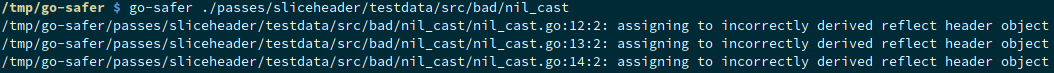
\includegraphics[width=\textwidth]{assets/images/chapter5/go-safer-screenshot.png}
    \caption{Usage example screenshot of \toolSafer{}}
    \label{fig:go-safer-screenshot}
    %\vspace{-14pt}
\end{figure}


\toolSafer{} is based on the same foundation as \toolVet{}, therefore it supports the same command line arguments and
options.
These include amongst others the option to include a context of adjacent source code lines for each warning in the
output, or change the output format to machine-readable JSON instead of the standard output, which is designed to be
read by humans.


%% ---------------------------------------------------------------------------------------------------------------------

\section{Implementation}\label{sec:go-safer:implementation}

As mentioned in the last section, \toolSafer{} is built using the Go analysis infrastructure that is available as part
of \toolVet{}.
This allows to compose analysis steps as modular and reusable parts, which are called \textit{passes}.
Each analysis pass is run on the source code packages under analysis as a unit.
It can depend on the results of other analysis passes, which are run before it and hand the results over to it.
The passes and their relations must form a directed acyclic graph, and the analyis infrastructure code determines the
optimal execution order and parallelism.
There are two novel analysis passes in \toolSafer{}, the \textit{sliceheader} and the \textit{structcast} pass.
Figure~\ref{fig:go-safer-architecture} shows an overview of this architecture.

\begin{figure}[!t]
    \vspace{2mm}
    \centering
    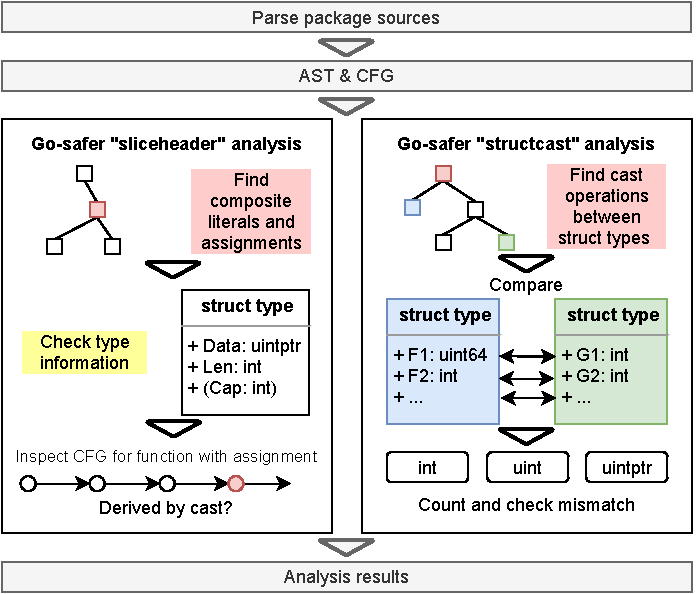
\includegraphics[width=0.48\textwidth]{gfx/figures/go-safer-architecture.pdf}
    %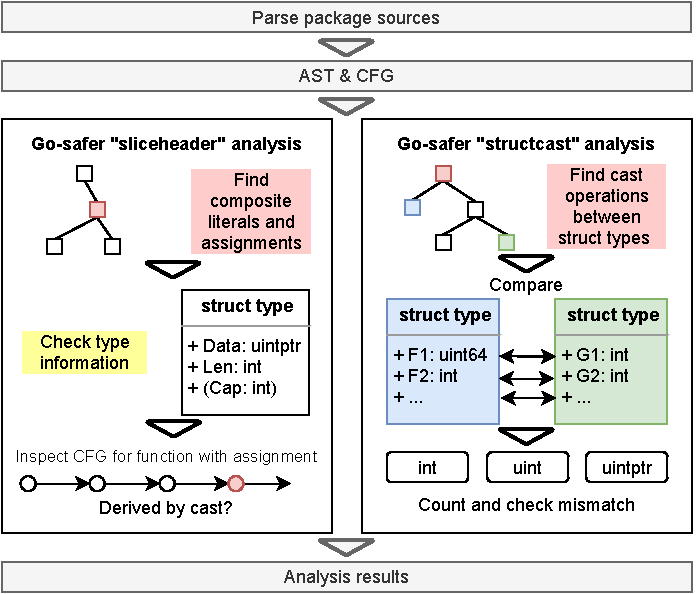
\includegraphics[width=0.45\textwidth]{gfx/figures/go-safer-architecture.pdf}
    \caption{Architecture of \toolSA{} static code analysis tool}
    \label{fig:safer-architecture}
    %\vspace{-14pt}
\end{figure}


Parsing the source code of the packages under analysis is done using the same code as \toolVet{} uses, in fact that code
is required as a dependency for \toolSafer{}.
Then, the abstract syntax tree (\acrshort{AST}) and control flow graph (\acrshort{CFG}) of the sources are built using
existing analysis passes which the novel \toolSafer{} passes depend upon.
After all analysis passes are finished, the results are also presented to the user by the same code used in \toolVet{}.
This composition using many existing parts allows to keep the required new code to a minimum, reuses well-tested pieces
of code, and allows integrating the new \toolSafer{} features into a familiar workflow.

The \textit{sliceheader} analysis pass first receives the \acrshort{AST} and filters it for composite literals and
assignment statements.
These are given by \textit{ast.CompositeLit} and \textit{ast.AssignStmt} nodes.
Recursively going down the \textit{AST} even after a composite literal has been found ensures that \toolSafer{} also
detects such literals that are part of a bigger structure type that contains a slice header as one of its fields.
Then, the type of either the composite literal or the assignment receiver is checked.
For assignments, this is done by looking up the left hand side identifier in a type table provided by the parser.
Since Go supports multiple assignments in one statement, there can be multiple variables on the left hand side.
In this case, \toolSafer{} checks all of them to see if any meets the conditions to trigger a warning.
To check whether the type matches either \textit{reflect.StringHeader} or \textit{reflect.SliceHeader}, the given type
is checked for assignability to the underlying structure of the header types.
This structure, as illustrated in Figure~\ref{fig:go-safer-architecture}, is one \textit{uintptr} field and one or two
\textit{int} fields.
Comparing to the structure instead of the name of the type makes it possible to detect type aliases to the header types
which might exist.
For example, when there is a \textit{type CustomHeader reflect.SliceHeader} definition, \toolSafer{} will also detect
composite literals of type \textit{CustomHeader}.
A composite literal of a header type is already enough to issue a warning, but for assignments \toolSafer{} needs to
check whether the receiver variable is a slice or string header that was created by conversion from a real slice or
string.
To do this, the \acrshort{AST} assignment node is located within the \acrshort{CFG}.
Then, going backwards in the \acrshort{CFG}, the last node that assigns the value of the receiver variable is found.
This node is the effective value of the slice or string header structure at the time of the assignment under
investigation.
Finally, \toolSafer{} checks whether the right hand side value of the statement defining that value is a conversion
from an actual slice or string value.
It has to be a cast through an \textit{unsafe.Pointer} value for this to be possible.
If that is the case, the assignment is legitimate and \toolSafer{} does not print a warning.
However, if the variable is not derived by a conversion from a slice or string, or no \acrshort{CFG} node defining the
variable can be found, a warning is issued.
This is possible, for example, if the slice or string header is passed in as a function parameter, because
its value can not be statically inferred with the Go analysis framework in that case.

The \textit{structcast} pass also uses the \acrshort{AST} to find cast operations.
These are represented in the \acrshort{AST} in the same way as function calls are, so the tree is filtered for
\textit{CallExpr} nodes.
If there is a cast from some structure type to \textit{unsafe.Pointer} and further to another structure type, these
source and target types are analyzed.
These types can again be fetched from a type lookup table provided by the parser.
For both of them, \toolSafer{} counts the number of fields that have the types \textit{int}, \textit{uint}, and
\textit{uintptr}.
These \checkNum{three} basic types are the ones available in Go that have different sizes on varying architectures.
For example, \textit{int} is \checkNum{eight} bytes on the \textit{amd64} architecture, but only \checkNum{four} bytes
on \textit{i386}.
If the counts mismatch, the direct cast using the \unsafe{} \acrshort{API} will likely break on some architectures,
and \toolSafer{} generates a warning.

A set of automated tests verifies that \toolSafer{} works as expected.
These tests also use the framework provided by the Go analysis infrastructure, which allows tests to be written as
individual source packages where expected warnings are given as line comments in the respective lines.
On the other hand, lines that must not trigger any warnings can either have no comment or an explicit \textit{ok}
comment.
This allows a fast and effective composition of new test cases.
At the same time, the test cases provide formal documentation about positive and negative examples for the code patterns
detected by \toolSafer{}.


%% ---------------------------------------------------------------------------------------------------------------------

\section{Evaluation}\label{sec:go-safer:evaluation}

In order to make a valuable contribution to the safety of Go programs and also be an effective tool for developers, it
is important that \toolSafer{} can find actual bugs in real-world Go projects, and at the same time has a low rate of
false positives and false negatives.
False negatives would mean that the tool misses incorrect and therefore potentially vulnerable usages of the \unsafe{}
\acrshort{API}.
On the other hand, a high rate of false positives would mean that it generates many warnings that are not related to
any programming errors.
This would require developers to manually review the findings and dismiss many of them, which decreases the value of
\toolSafer{} significantly.
First, developers could lose trust in the tool and refuse using it with their regular development workflows.
Second, false positives make it hard to integrate \toolSafer{} with automated \acrshort{CI} processes, because the build
would fail without there being a real problem.

To demonstrate that \toolSafer{} is capable of findings actual bugs while having an acceptable rate of both false
positives and negatives, its performance is evaluated in two different ways.
One of them uses the novel data set of labeled \unsafe{} usages, which was presented in
Section~\ref{sec:go-geiger:labeled-dataset}.
The second one is done by manually analyzing \checkNum{six} selected open-source Go packages from different projects and
comparing the results to the output of \toolSafer{}.
As shown in the following sections, \toolSafer{} is able to achieve both high precision and accuracy in the two
evaluations.
Finally, the performance is compared to the existing static analysis tools \toolVet{} and \toolGosec{}.

In addition to this academic evaluation, \toolSafer{} was also used to discover more than \numberBugsFixedRounded{} bugs
that existed in the open-source projects used for the study on real-world usage of \unsafe{} presented in
Chapter~\ref{ch:go-geiger} or their dependencies.


%% ---------------------------------------------------------------------------------------------------------------------

\subsection{Labeled Usages}\label{subsec:go-safer:evaluation:labeled-usages}

To evaluate the performance of \toolSafer{} using the novel data set of labeled \unsafe{} usages, first all instances
with the label \textit{cast-header} are taken from the set.
These are possible misuses involving incorrect constructions of slice and string headers.
There are \checkNum{44} such code samples, which are manually classified as positive and negative examples.
Positive means that the code is a misuse of the \unsafe{} \acrshort{API} and \toolSafer{} should generate a warning for
it, while negative means that the code is a correct and safe usage.
There are \checkNum{30} positive and \checkNum{14} negative samples.

Then, \toolSafer{} is run on all packages that contain the respective \checkNum{44} \unsafe{} usage samples, and all
warnings issued are saved into a \acrshort{CSV} file.
This makes it easy to match the warnings with the labeled samples by their file name and line number.
Samples that are classified as positive are counted as true positives (TP) if \toolSafer{} generated a warning for it,
and false positives (FP) otherwise.
Similarly, negative samples count as false negatives (FN) if there is a warning, and true negatives (TN) otherwise.
Table~\ref{tbl:go-safer-evaluation-dataset} shows the results of this evaluation in its first line.
The other lines contain results from other linters and are discussed in
Section~\ref{subsec:go-safer:evaluation:linters-comparison}.
Furthermore, the table contains the resulting precision, recall, accuracy, and F1-score as calculated from the classes
counts.

\begin{table}[htp!]
    \centering
    \caption{Evaluation results for \toolSafer{} on the labeled data set of \unsafe{} usages}
    \label{tbl:gosafer-evaluation-dataset}
    \begin{tabular}{l||r|r|r|r||l|l|l|l}
        \textbf{Tool} & \textbf{TP} & \textbf{FP} & \textbf{TN} & \textbf{FN} & \textbf{Precision} & \textbf{Recall} & \textbf{Accuracy} & \textbf{F1-Score} \\
        \hline
        go-safer &   29   &    1   &   13   &    1   &   0.967       &  0.967     &    0.955     & 0.967  \\
        go vet   &    0   &    0   &   14   &   30   &   -           &  0         &    0.318     & 0      \\
        gosec    &   29   &   13   &    1   &    1   &   0.690       &  0.967     &    0.681     & 0.805  \\
    \end{tabular}
\end{table}

The results show both high precision and recall of \checkNum{96.7\%} for \toolSafer{}.
High precision means that there are few false positives, so the warnings generated by \toolSafer{} are almost always
correct and show evidence of an actual bug in the code.
Therefore, developers can include it into their workflows without the need of dismissing many invalid warnings.
A high recall shows that there are few false negatives, therefore a high fraction of the existing bugs is detected by
\toolSafer{}.
Developers thus have a reliable tool at hand to be trusted in detecting bugs of the particular class of \unsafe{}
misuses that it is specialized in.
Accuracy and F1-score are high as well, which follows from both high precision and recall and emphasizes the quality
\toolSafer{} provides.

A manual analysis shows that the false positive is due to a slice header that is created from a real slice, however
the slice is referenced through a slightly obfuscated, reflected pointer which \toolSafer{} can not connect to the
slice.
The false negative is caused by compilation errors in the package which prevent \toolSafer{} from analyzing the package
altogether.
Since it depends on the \acrshort{AST}, its static analysis passes can not run and the execution stops with a generic
error message before the parsing step has finished.
To work around this scenario, \toolSafer{} would need a secondary analysis strategy that works on the source code
instead of the \acrshort{AST}, which is not feasible.


%% ---------------------------------------------------------------------------------------------------------------------

\subsection{Case Studies}\label{subsec:go-safer:evaluation:case-studies}

A second evaluation of \toolSafer{} is done by manually analyzing \checkNum{six} selected Go packages from open-source
projects.
These packages are chosen using the results of the study on \unsafe{} usage in open-source code presented in
Chapter~\ref{ch:go-geiger}.
Evaluating \toolSafer{}, an \unsafe{}-related linter, on packages that do not actually contain any \unsafe{} usages does
not provide valuable insights.
Table~\ref{tbl:go-safer-evaluation-packages-stats} shows the \checkNum{six} packages used for this evaluation, including
their number of Go files, lines of code, and \unsafe{} usages.
To create a variation both of the amount of \unsafe{} and package size, they are selected to include two packages
each with few, medium, and many \unsafe{} usages.
For every category, there is one small and one large package each.

\begin{table}[htp!]
    \centering
    \caption{Selected packages for the evaluation of \toolSafer{}}
    \label{tbl:go-safer-evaluation-packages-stats}
    \begin{tabular}{l|r|r|r}
        \textbf{Package}                        & \textbf{Number of Go Files} & \textbf{\acrshort{LOC}} & \textbf{Unsafe Usages} \\
        \hline
        k8s.io/kubernetes/pkg/apis/core/v1      & 6                           & 10,048                  & 677                    \\
        \rowcolor{verylightgray}
        gorgonia.org/tensor/native              & 4                           & 1,867                   & 158                    \\
        github.com/anacrolix/mmsg/socket        & 86                          & 3,782                   & 115                    \\
        \rowcolor{verylightgray}
        github.com/cilium/ebpf                  & 14                          & 2,851                   & 65                     \\
        golang.org/x/tools/internal/event/label & 1                           & 213                     & 8                      \\
        \rowcolor{verylightgray}
        github.com/mailru/easyjson/jlexer       & 4                           & 1,234                   & 5                      \\
        \hline
        \textbf{Total}                          & \textbf{115}                & \textbf{19,995}         & \textbf{1,028}         \\
    \end{tabular}
\end{table}

The \checkNum{six} packages were analyzed manually to find any insecure code that \toolSafer{} should detect.
The results of this were saved as a \acrshort{CSV} file containing a positive or negative label for every line of code
that includes a usage of the \unsafe{} \acrshort{API}.
Lines that do not use the \acrshort{API} should not be analyzed by \toolSafer{} at all, therefore they are not included
as negative in order to avoid a very large number of true negatives which would skew the accuracy and yield less
valuable evaluation results.
Should \toolSafer{} generate a warning for such a line, it will still be counted as false positive.
After the manual analysis, \toolSafer{} was run on the packages and all warnings were saved again.
Similar to Section~\ref{subsec:go-safer:evaluation:labeled-usages}, the warnings and labels were matched and counted.
Table~\ref{tbl:go-safer-evaluation-packages} shows the results of the evaluation for each package individually as well
as in total.
The numbers for \toolSafer{} are in the first column for each value (Tool~\textit{a}), while the other two columns are
discussed in the following section for a comparison to existing linters again.

\begin{table}[htp!]
    \centering
    \caption[Evaluation results for \toolSafer{} on manually analyzed packages packages]
        {Evaluation results for \toolSafer{} on manually analyzed packages packages~\newline \tiny ~\newline \footnotesize
        Tools: \underline{a} \toolSafer{}, \underline{b} \toolVet{}, \underline{c} \toolGosec{} \tiny ~\newline}
    \label{tbl:go-safer-evaluation-packages}
    \begin{adjustbox}{max width=\textwidth}
        \begin{tabular}{l||rrr|rrr|rrr|rrr||lll|lll|lll|lll}
            \textbf{Package} & \multicolumn{3}{c|}{\textbf{TP}}                & \multicolumn{3}{c|}{\textbf{FP}}                   & \multicolumn{3}{c|}{\textbf{TN}}                    & \multicolumn{3}{c||}{\textbf{FN}}                  & \multicolumn{3}{c|}{\textbf{Precision}}  & \multicolumn{3}{c|}{\textbf{Recall}}    & \multicolumn{3}{c|}{\textbf{Accuracy}}           & \multicolumn{3}{c}{\textbf{F1-Score}}    \\
            {}               & \textit{a}            & \textit{b} & \textit{c} & \textit{a}             & \textit{b} & \textit{c}   & \textit{a}            & \textit{b}   & \textit{c}   & \textit{a}             & \textit{b}  & \textit{c}  & \textit{a}     & \textit{b} & \textit{c} & \textit{a}    & \textit{b} & \textit{c} & \textit{a}     & \textit{b}     & \textit{c}     & \textit{a}     & \textit{b} & \textit{c} \\
            \hline
            v1               & 0                     & 0          & 0          & 0                      & 0          & 676          & 677                   & 677          & 1            & 0                      & 0           & 0           & -              & -          & 0          & -             & -          & -          & 1              & 1              & 0.001          & -              & -          & -          \\
            \rowcolor{verylightgray}
            native           & 48                    & 0          & 0          & 9                      & 0          & 98           & 101                   & 110          & 12           & 0                      & 48          & 48          & 0.842          & -          & 0          & 1             & 0          & 0          & 0.943          & 0.696          & 0.076          & 0.914          & -          & -          \\
            socket           & 0                     & 0          & 0          & 0                      & 0          & 16           & 115                   & 115          & 99           & 0                      & 0           & 0           & -              & -          & 0          & -             & -          & -          & 1              & 1              & 0.861          & -              & -          & -          \\
            \rowcolor{verylightgray}
            ebpf             & 0                     & 0          & 0          & 1                      & 0          & 38           & 64                    & 65           & 27           & 0                      & 0           & 0           & 0              & -          & 0          & -             & -          & -          & 0.985          & 1              & 0.415          & -              & -          & -          \\
            label            & 0                     & 0          & 0          & 0                      & 0          & 7            & 8                     & 8            & 1            & 0                      & 0           & 0           & -              & -          & 0          & -             & -          & -          & 1              & 1              & 0.125          & -              & -          & -          \\
            \rowcolor{verylightgray}
            jlexer           & 1                     & 0          & 0          & 0                      & 0          & 2            & 4                     & 4            & 2            & 0                      & 1           & 1           & 1              & -          & 0          & 1             & 0          & 0          & 1              & 0.8            & 0.4            & 1              & -          & -          \\
            \hline
            \textbf{Total}   & \textbf{49}           & \textbf{0} & \textbf{0} & \textbf{10}            & \textbf{0} & \textbf{837} & \textbf{969}          & \textbf{979} & \textbf{142} & \textbf{0}             & \textbf{49} & \textbf{49} & \textbf{0.831} & \textbf{-} & \textbf{0} & \textbf{1}    & \textbf{0} & \textbf{0} & \textbf{0.990} & \textbf{0.952} & \textbf{0.138} & \textbf{0.907} & \textbf{-} & \textbf{-} \\
        \end{tabular}
    \end{adjustbox}
\end{table}

In this second evaluation, \toolSafer{} demonstrates a slightly lower precision of \checkNum{83.1\%}, which means that
about \checkNum{one} in \checkNum{six} warnings is a false positive.
The recall however is at \checkNum{100\%}, resulting in a still excellent accuracy of \checkNum{99\%} and F1-score of
\checkNum{90.7\%}.

The false positives generated by \toolSafer{} for the \textit{native} package are caused by the same reasoning as the
false positive described in the previous section, but this time all of the occurrences of that pattern in the package
are found.
For the \textit{ebpf} package, the false positive is an exact match of the detection rules implemented by \toolSafer{},
however in that particular case the usage is not vulnerable to the possible \textit{use-after-free} bug described before
because a call to the \textit{runtime.KeepAlive} function prevents the underlying data array referenced in the created
slice header from being freed when the garbage collector runs.
\toolSafer{} does not detect this, which is a limitation of its rule set.


%% ---------------------------------------------------------------------------------------------------------------------

\subsection{Comparison with Existing Tools}\label{subsec:go-safer:evaluation:linters-comparison}

In this section, the performance of \toolSafer{} is compared to the previously existing static analysis tools \toolVet{}
and \toolGosec{}.
For both evaluation sets described in the previous sections, these tools were also run and their respective generated
warnings were saved.
This allows to identify true and false positives and negatives in the same way as for \toolSafer{}.
However, only the respective warnings that are related to the \unsafe{} \acrshort{API} are counted.
For \toolVet{}, this is the \textit{"possible misuse of unsafe.Pointer"} message generated by the \textit{unsafeptr}
pass, and for \toolGosec{} it is rule \checkNum{\textit{G103}} resulting in the \textit{"use of unsafe should be
audited"} message.

The results are presented in Tables~\ref{tbl:go-safer-evaluation-dataset} and~\ref{tbl:go-safer-evaluation-packages}
next to those of \toolSafer{}, in the remaining two lines and columns \textit{b} and~\textit{c}, respectively.
Both evaluations, on the labeled data set and \checkNum{six} manually analyzed packages, reveal that \toolVet{} did not
generate any \unsafe{}-related warnings, while \toolGosec{} simply flagged all usages of \unsafe{} as potentially
dangerous.
The \toolGosec{} results contain some false negatives because there are code lines in the evaluation data set that do
not contain a direct call of a function belonging to the \unsafe{} package.
These are assignments to slice and string headers which are previously created, which are detected by \toolSafer{} but
not \toolGosec{}.
Similarly, there are no true positives for \toolGosec{} in Table~\ref{tbl:go-safer-evaluation-packages} because there
are no positive samples in that evaluation set that contain a direct usage of \textit{unsafe.Pointer} in the line of
code.

The reported performance metrics are not very meaningful for \toolVet{} and \toolGosec{}.
With the evaluation on the labeled data set of \unsafe{} usages shown in Table~\ref{tbl:go-safer-evaluation-dataset},
\toolVet{} has a low accuracy of \checkNum{31.8\%} although precision and recall are not defined.
This accuracy simply mirrors the fraction of negative samples in the overall sample set.
Similarly, the inverse of that fraction (\checkNum{68.1\%}) is seen as the accuracy of \toolGosec{} in that table.
It also has a rather high precision and recall but this is simply the result of generating warnings for every sample in
the set.
In the second evaluation on the \checkNum{six} packages, none of them achieves a defined and greater than zero precision
or recall for either \toolVet{} or \toolGosec{} because both tools do not report any true positives.
However, \toolVet{} still gets a high accuracy of \checkNum{95.2\%} because this evaluation set contains a lot more
negative samples than positve ones.

In summary, this comparison shows that neither \toolVet{} nor \toolGosec{} are suitable for the purpose that
\toolSafer{} fulfills, the tools achieve different goals.


%% ---------------------------------------------------------------------------------------------------------------------

\section{Summary}\label{sec:go-safer:summary}

\todo{write summary}
